\documentclass{standalone}
\usepackage{tikz}
\usepackage{ctex,siunitx}
\setCJKmainfont{Noto Serif CJK SC}
\usepackage{tkz-euclide}
\usepackage{amsmath}
\usetikzlibrary{patterns, calc,3d}
\usetikzlibrary {decorations.pathmorphing,decorations.pathreplacing,decorations.shapes}
\begin{document}
\small
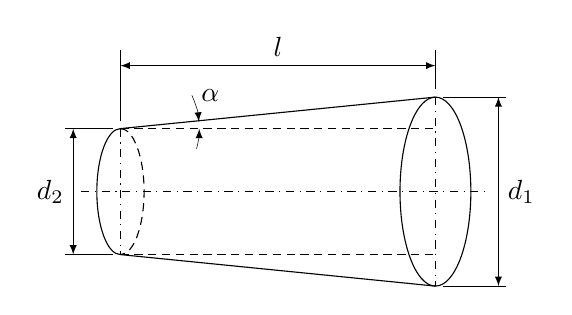
\begin{tikzpicture}[>=latex]
  \draw[dashdotted](-0.5,0)--(4.7,0)(0,0.8)--(0,-0.8)(4,1.2)--(4,-1.2);
  \draw(0,0.8)arc(90:270:0.3 and 0.8);
  \draw[densely dashed](0,0.8)arc(90:-90:0.3 and 0.8);
  \draw(4,0)ellipse(0.45 and 1.2);
  % \draw[densely dashed](4,1.2)arc(90:-90:0.45 and 1.2);
  \draw(0,0.8)--(4,1.2)(0,-0.8)--(4,-1.2);
  \draw[densely dashed](0,0.8)--(4,0.8)(0,-0.8)--(4,-0.8);
  \draw[very thin,<-](1,0.8)arc(0:-15:1);
  \draw[very thin,<-]([shift=(5:1)]0,0.8)arc(5:25:1)node[right]{$\alpha$};
  \draw[very thin](0,0.9)--(0,1.8)(4,1.3)--(4,1.8)(-0.1,0.8)--(-0.7,0.8)(-0.1,-0.8)--(-0.7,-0.8)(4.1,1.2)--(4.9,1.2)(4.1,-1.2)--(4.9,-1.2);
  \draw[very thin,<->](0,1.6)--(4,1.6)node[midway,above]{$l$};
  \draw[very thin,<->](-0.6,-0.8)--(-0.6,0.8)node[midway,left]{$d_2$};
  \draw[very thin,<->](4.8,-1.2)--(4.8,1.2)node[midway,right]{$d_1$};
\end{tikzpicture}
\end{document}